% ============================================================
%  N-Body Simulation — GPU Computing Report
%  Grenoble INP — Ensimag
% ============================================================

\documentclass[12pt, a4paper]{article}

\usepackage[T1]{fontenc}
\usepackage[utf8]{inputenc}
\usepackage[english]{babel}
\usepackage[top=2.5cm, bottom=2.5cm, left=2.8cm, right=2.8cm, headheight=15pt]{geometry}
\usepackage{setspace}
\onehalfspacing

\usepackage{fancyhdr}
\pagestyle{fancy}
\fancyhf{}
\fancyhead[L]{\small\textit{N-Body Simulation --- GPU Computing}}
\fancyhead[R]{\small\textit{Ensimag 3A}}
\fancyfoot[C]{\thepage}
\renewcommand{\headrulewidth}{0.4pt}

\usepackage{amsmath, amssymb}
\usepackage{booktabs}
\usepackage{array}
\usepackage{graphicx}
\usepackage{float}
\usepackage{caption}
\usepackage{tikz}
\usetikzlibrary{arrows.meta, positioning}
\usepackage[colorlinks=true, linkcolor=black, citecolor=black, urlcolor=blue]{hyperref}
\usepackage{enumitem}
\usepackage{parskip}
\usepackage{xcolor}
\usepackage{listings}

\definecolor{codebg}{RGB}{248,248,248}
\definecolor{codeframe}{RGB}{210,210,210}
\definecolor{kw}{RGB}{0,0,180}
\definecolor{cm}{RGB}{60,120,60}

\lstdefinestyle{cuda}{
  backgroundcolor=\color{codebg},
  frame=single, rulecolor=\color{codeframe},
  basicstyle=\ttfamily\small,
  keywordstyle=\color{kw}\bfseries,
  commentstyle=\color{cm}\itshape,
  numberstyle=\tiny\color{gray},
  numbers=left, numbersep=8pt, stepnumber=1,
  tabsize=4, showstringspaces=false,
  breaklines=true, captionpos=b,
  language=C++,
  morekeywords={__global__, __shared__, __device__, __host__, __restrict__,
                __syncthreads, threadIdx, blockIdx, blockDim,
                cudaMalloc, cudaFree, cudaMemcpy, cudaMemcpyAsync,
                cudaHostAlloc, cudaFreeHost, cudaStreamCreate,
                cudaStreamSynchronize, cudaDeviceSynchronize,
                cudaGetLastError, cudaMemcpyHostToDevice,
                cudaMemcpyDeviceToHost, cudaHostAllocDefault,
                rsqrtf, __ldg, uint32_t},
}
\lstset{style=cuda}

% ── Title metadata ───────────────────────────────────────────
\newcommand{\StudentName}{BODIN Jules}
\newcommand{\Program}{3rd year -- M2 AI}
\newcommand{\ReportDate}{February 2026}

% ============================================================
\begin{document}
% ============================================================

\begin{titlepage}
\centering
\vspace*{1.8cm}
{\Large \textsc{Grenoble INP -- Ensimag}\\[0.4em] \large \Program}

\vspace{1.8cm}
\rule{\linewidth}{0.5pt}\\[0.5em]
{\LARGE \textbf{N-Body Simulation}}\\[0.4em]
{\large CPU/GPU Hybrid Implementation with Barnes-Hut}\\[0.4em]
\rule{\linewidth}{0.5pt}

\vspace{1.4cm}
{\large GPU Computing --- Project Report}

\vspace{3cm}
\begin{tabular}{rl}
  \textbf{Author:}     & \StudentName \\[0.4em]
  \textbf{Date:}       & \ReportDate  \\
\end{tabular}

\end{titlepage}

\tableofcontents
\newpage

% ============================================================
\section{Introduction}
% ============================================================

The N-body problem simulates the gravitational dynamics of $N$ point masses. The net acceleration of body $i$ is:

\begin{equation}
  \mathbf{a}_i = G \sum_{j \neq i}
    \frac{m_j \,(\mathbf{r}_j - \mathbf{r}_i)}
         {\bigl(\|\mathbf{r}_j - \mathbf{r}_i\|^2 + \varepsilon^2\bigr)^{3/2}}
  \label{eq:accel}
\end{equation}

where $\varepsilon$ is a softening parameter that prevents singularities at close range. Direct evaluation is $\mathcal{O}(N^2)$ per step, which limits interactive simulations to $N \lesssim 10^4$ on a CPU.

\paragraph{N-body units.}
The simulator uses $G = 1$ throughout, which corresponds to the standard N-body unit system~\cite{heggie1986}. In this system, units of length, mass, and time are chosen so that $G = 1$ and the total mass $M = 1$, keeping all dynamically relevant quantities of order unity. This convention eliminates the numerical constant from equation~\eqref{eq:accel} and avoids the floating-point scaling issues that arise with SI units, where $G \approx 6.674 \times 10^{-11}$ would require careful rescaling of masses and distances to prevent underflow or overflow. It is the standard choice in gravitational N-body codes.

This project implements an N-body simulator in Rust with two algorithms (direct $N^2$ and Barnes-Hut) on two backends (CPU and GPU). The GPU kernels are written in CUDA C++ in \texttt{kernel.cu} and \texttt{barnes\_hut.cu}, compiled by \texttt{nvcc} and called from Rust via an \texttt{extern "C"} FFI boundary. The focus of this report is the GPU implementation and the optimizations that make Barnes-Hut efficient on SIMT hardware.

% ============================================================
\section{Algorithms}
% ============================================================

\subsection{Direct $N^2$}

Every body computes its interaction with all $N-1$ others: one thread per body, independent computations, no data dependencies. The kernel in \texttt{kernel.cu} uses \texttt{blockSize = 256} and a standard grid layout:

\begin{lstlisting}[caption={$N^2$ kernel signature and grid launch (\texttt{kernel.cu}, lines 10--22, 143--154).}]
__global__ void compute_forces_nsquare(
    const float * __restrict__ pos_x,
    const float * __restrict__ pos_y,
    const float * __restrict__ masses,
    float       * __restrict__ acc_x,
    float       * __restrict__ acc_y,
    int n, float epsilon_sq, float G)
{
    int i = blockIdx.x * blockDim.x + threadIdx.x;
    if (i >= n) return;
    ...
    float inv_r  = rsqrtf(dist_sq + epsilon_sq);
    float inv_r3 = inv_r * inv_r * inv_r;
    float factor = G * masses[j] * inv_r3;
}
// Launch:
int blockSize = 256;
int gridSize  = (n + blockSize - 1) / blockSize;
compute_forces_nsquare<<<gridSize, blockSize>>>(...);
\end{lstlisting}

This algorithm is embarrassingly parallel with high arithmetic intensity, so it scales well on GPU without any shared memory optimization.

\subsection{Barnes-Hut}

Barnes-Hut reduces complexity to $\mathcal{O}(N \log N)$ by approximating groups of distant bodies as a single mass. The domain is recursively subdivided into a quadtree (2D) or octree (3D). For each body, the tree is traversed: a cell of geometric size $s$ at distance $d$ is treated as a single point mass if

\begin{equation}
  \frac{s}{d} < \theta
  \label{eq:opening}
\end{equation}

The parameter $\theta$ (default 1.0) controls the accuracy-performance tradeoff. The implementation supports both 2D and 3D via compile-time flags \texttt{-DVEC2} / \texttt{-DVEC3}.

% ============================================================
\section{CUDA Implementation}
% ============================================================

\subsection{Hybrid CPU/GPU Design}

Tree construction has fundamental sequential data dependencies: inserting body $B$ may require subdividing a leaf created by body $A$. It therefore runs on the CPU. Force computation is independent across bodies and runs on the GPU. This hybrid design avoids the complexity of a fully GPU-resident construction algorithm while keeping the dominant cost (force evaluation) massively parallel.

\subsection{Per-Step Pipeline}

Figure~\ref{fig:pipeline} shows the complete data flow for one Barnes-Hut GPU step, as implemented in \texttt{cuda\_barnes\_hut\_forces()} in \texttt{barnes\_hut.cu} (lines 687--875).

\begin{figure}[H]
\centering
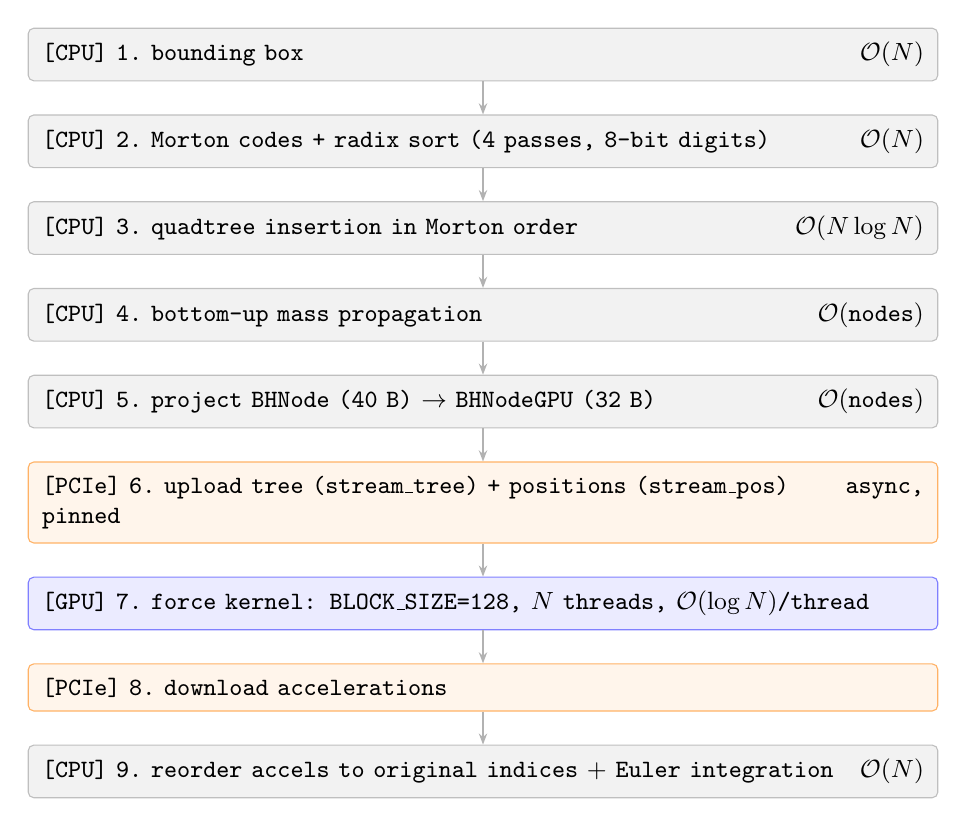
\begin{tikzpicture}[
  node distance=0.42cm,
  cpu/.style  = {rectangle, draw=gray!50,   fill=gray!10,   rounded corners=2pt,
                 text width=11.2cm, align=left, font=\small\ttfamily, inner sep=5pt},
  gpu/.style  = {rectangle, draw=blue!50,   fill=blue!8,    rounded corners=2pt,
                 text width=11.2cm, align=left, font=\small\ttfamily, inner sep=5pt},
  pcie/.style = {rectangle, draw=orange!60, fill=orange!8,  rounded corners=2pt,
                 text width=11.2cm, align=left, font=\small\ttfamily, inner sep=5pt},
  arr/.style  = {-{Stealth[length=4pt]}, gray!60, line width=0.7pt}
]
\node[cpu] (bb)   {[CPU]  1.\ bounding box \hfill $\mathcal{O}(N)$};
\node[cpu,  below=of bb]   (ms)   {[CPU]  2.\ Morton codes + radix sort (4 passes, 8-bit digits) \hfill $\mathcal{O}(N)$};
\node[cpu,  below=of ms]   (ins)  {[CPU]  3.\ quadtree insertion in Morton order \hfill $\mathcal{O}(N \log N)$};
\node[cpu,  below=of ins]  (prop) {[CPU]  4.\ bottom-up mass propagation \hfill $\mathcal{O}(\text{nodes})$};
\node[cpu,  below=of prop] (ext)  {[CPU]  5.\ project BHNode (40 B) $\to$ BHNodeGPU (32 B) \hfill $\mathcal{O}(\text{nodes})$};
\node[pcie, below=of ext]  (upl)  {[PCIe] 6.\ upload tree (stream\_tree) + positions (stream\_pos) \hfill async, pinned};
\node[gpu,  below=of upl]  (ker)  {[GPU]  7.\ force kernel: BLOCK\_SIZE=128, $N$ threads, $\mathcal{O}(\log N)$/thread};
\node[pcie, below=of ker]  (dnl)  {[PCIe] 8.\ download accelerations};
\node[cpu,  below=of dnl]  (rei)  {[CPU]  9.\ reorder accels to original indices $+$ Euler integration \hfill $\mathcal{O}(N)$};

\draw[arr](bb)--(ms); \draw[arr](ms)--(ins); \draw[arr](ins)--(prop);
\draw[arr](prop)--(ext); \draw[arr](ext)--(upl); \draw[arr](upl)--(ker);
\draw[arr](ker)--(dnl); \draw[arr](dnl)--(rei);
\end{tikzpicture}
\caption{Per-step pipeline (\texttt{cuda\_barnes\_hut\_forces}, \texttt{barnes\_hut.cu}).
  Grey = CPU, blue = GPU, orange = PCIe transfer.}
\label{fig:pipeline}
\end{figure}

\subsection{Skip Pointers and Traversal Sentinel}

Rather than a recursive traversal, each tree node stores two navigation fields (declared in \texttt{BHNode} and mirrored in \texttt{BHNodeGPU}):
\begin{itemize}[noitemsep]
  \item \texttt{children}: index of the first child (0 = leaf);
  \item \texttt{next}: index of the next node after skipping this entire subtree.
\end{itemize}

When the opening criterion (equation~\ref{eq:opening}) is satisfied, the traversal jumps to \texttt{node.next} in $O(1)$, with no recursive call and no stack. The root is initialized with \texttt{next = -1} as an end-of-traversal sentinel (line 784 of \texttt{barnes\_hut.cu}). Using $-1$ rather than $0$ is deliberate: the root itself has index 0, so a link to $0$ would be indistinguishable from a valid back-edge.

The traversal loop in the GPU kernel terminates when \texttt{node < 0}:

\begin{lstlisting}[caption={Traversal loop with skip pointers (\texttt{barnes\_hut.cu}, lines 524--561).}]
int node = 0;
while (node >= 0) {
    BHNodeGPU nd = (node < to_load) ? smem[node] : nodes[node];
    if (nd.mass == 0.0f) { node = nd.next; continue; }

    float cell_sq = (nd.half_size * 2.0f) * (nd.half_size * 2.0f);
    bool  is_leaf = (nd.children == 0);
    bool  is_far  = (cell_sq < dist_sq * theta_sq);

    if (is_leaf || is_far) {
        float inv_r  = rsqrtf(dist_sq + epsilon_sq);
        float inv_r3 = inv_r * inv_r * inv_r;
        float f = G * nd.mass * inv_r3;
        ax += dx * f;  ay += dy * f;
        node = nd.next;      // skip (or end if -1)
    } else {
        node = nd.children;  // descend
    }
}
\end{lstlisting}

% ============================================================
\section{Optimizations}
% ============================================================

\subsection{Morton Curve Sorting}
\label{sec:morton}

\subsubsection{Problem: Warp Divergence}

The primary bottleneck of GPU Barnes-Hut is warp divergence. 32 threads form a warp and execute in SIMT lockstep. Without spatial ordering, two adjacent threads may process bodies on opposite sides of the domain and follow completely different paths through the tree. The warp must serialize all divergent branches, leaving most threads idle. In practice, warp efficiency without sorting is around 12\% (4 active threads out of 32), which gives essentially no speedup over a single CPU thread.

\subsubsection{Solution: Z-Order Curve}

The Morton code maps a multidimensional coordinate to a 1D integer while preserving spatial locality. Bodies that are close in space receive similar Morton indices. By sorting bodies by Morton code before tree construction, adjacent threads in a warp process spatially adjacent bodies and follow nearly identical traversal paths, driving warp divergence close to zero.

Each coordinate is quantized to 10 bits in $[0, 1023]$ and the bits of $x$ and $y$ are interleaved:

\begin{lstlisting}[caption={Bit expansion and 2D Morton encoding (\texttt{barnes\_hut.cu}, lines 366--406).}]
static inline uint32_t expand_bits_2d(uint32_t v) {
    v = (v | (v << 16)) & 0x0000FFFF;
    v = (v | (v <<  8)) & 0x00FF00FF;
    v = (v | (v <<  4)) & 0x0F0F0F0F;
    v = (v | (v <<  2)) & 0x33333333;
    v = (v | (v <<  1)) & 0x55555555;
    return v;
}
// Result: ...iy[1] ix[1] iy[0] ix[0]
uint32_t ix = (uint32_t)fminf(1023.f, (x - min_x) * inv_rx * 1023.f);
uint32_t iy = (uint32_t)fminf(1023.f, (y - min_y) * inv_ry * 1023.f);
return (expand_bits_2d(iy) << 1) | expand_bits_2d(ix);
\end{lstlisting}

The sort is a 32-bit LSD radix sort with 8-bit digits over 4 passes (stable, $\mathcal{O}(N)$, faster than \texttt{qsort} for $N > 10\,000$). After 4 passes (an even number), the result is in the original buffers with no final copy needed:

\begin{lstlisting}[caption={Radix sort structure (\texttt{barnes\_hut.cu}, lines 423--453).}]
for (int pass = 0; pass < 4; pass++) {
    int shift = pass * 8;
    int hist[256] = {};
    for (int i = 0; i < n; i++)
        hist[(keys[i] >> shift) & 0xFF]++;
    // prefix sum -> scatter
    ...
    // swap src/dst buffers each pass
    int* ti = idx; idx = tmp_idx; tmp_idx = ti;
}
// After 4 (even) passes: result is back in original buffers
\end{lstlisting}

Since the GPU kernel computes accelerations in Morton order, they are remapped to original body indices after the download (step 9 of the pipeline, lines 857--874 of \texttt{barnes\_hut.cu}) using the sort index array \texttt{g\_sort\_idx}.

\subsection{Compact GPU Node Structure}

The full \texttt{BHNode} struct used for CPU construction contains fields only needed during insertion: the geometric cell center \texttt{cx}, \texttt{cy} (and \texttt{cz} in 3D) used to determine child quadrants. These are never accessed during force traversal and should not be sent to the GPU.

Before upload, each node is projected into a compact \texttt{BHNodeGPU}:

\begin{lstlisting}[caption={The two node structs (\texttt{barnes\_hut.cu}, lines 65--103).}]
struct BHNode {                  // CPU construction: ~40 bytes
    float px, py, mass;
    int   children, next;
    float cx, cy;                // geometric center -- construction only
    float half_size;
};

struct __align__(16) BHNodeGPU { // GPU kernel: 32 bytes
    float px, py, mass;
    int   children, next;
    float half_size;
    float _pad[2];               // pad to 32-byte memory transaction
};
\end{lstlisting}

The \texttt{\_\_align\_\_(16)} declaration and explicit padding align each node to a 32-byte memory transaction, reducing the number of transactions per access. This cuts PCIe transfer volume by $\approx$20\% and proportionally reduces L1 cache pressure during traversal.

\subsection{Shared Memory for Upper Tree Levels}

Every thread visits the root and the upper levels of the tree on every traversal. Loading these from DRAM costs 200--400 cycles of latency per access. Instead, the first \texttt{SHARED\_NODES} nodes are cooperatively preloaded into shared memory at block launch:

\begin{lstlisting}[caption={Cooperative SMEM preload (\texttt{barnes\_hut.cu}, lines 499--507).}]
__shared__ BHNodeGPU smem[SHARED_NODES];
int to_load = min(SHARED_NODES, node_count);
for (int k = tid; k < to_load; k += BLOCK_SIZE)
    smem[k] = nodes[k];
__syncthreads();
\end{lstlisting}

\texttt{SHARED\_NODES} covers the first complete tree levels (defined at lines 56--59):

\begin{center}
\begin{tabular}{lllll}
  \toprule
  Mode & Branching & Levels & Nodes & SMEM/block \\
  \midrule
  \texttt{VEC2} & 4 & 0--3 & $1+4+16+64=85$ & $85\times32=2720$ B \\
  \texttt{VEC3} & 8 & 0--2 & $1+8+64=73$    & $73\times32=2336$ B \\
  \bottomrule
\end{tabular}
\end{center}

Both values are well below the 48 KB per-SM shared memory limit, preserving full occupancy. During traversal, nodes below \texttt{to\_load} are served from SMEM (4-cycle latency); deeper nodes fall back to global memory through the read-only L1 cache (line 525):

\begin{lstlisting}[caption={SMEM/global select during traversal (\texttt{barnes\_hut.cu}, line 525).}]
BHNodeGPU nd = (node < to_load) ? smem[node] : nodes[node];
\end{lstlisting}

\subsection{Block Size: 128 vs.\ 256}

The Barnes-Hut force kernel uses \texttt{BLOCK\_SIZE = 128} (line 53 of \texttt{barnes\_hut.cu}), while the $N^2$ kernel in \texttt{kernel.cu} uses 256. The difference reflects register pressure: the BH kernel maintains a traversal pointer, two accumulated force components, six per-node distance values, and intermediate boolean flags across the entire while loop. At 256 threads per block, this register footprint exceeds the per-SM budget, causing register spilling to slow local memory. At 128, all values remain in registers and occupancy is maximized on Turing and Ampere architectures.

\subsection{Pinned Memory and Asynchronous Transfers}

By default, \texttt{cudaMemcpy} from pageable host memory requires the runtime to stage data through an internal pinned buffer, adding one full CPU-side copy. The sorted position arrays and the compact tree are therefore allocated with \texttt{cudaHostAlloc} (page-locked memory):

\begin{lstlisting}[caption={Pinned allocation (\texttt{barnes\_hut.cu}, lines 631--651).}]
cudaHostAlloc(&g_gpu.h_sorted_px, s, cudaHostAllocDefault);
cudaHostAlloc(&g_gpu.h_sorted_py, s, cudaHostAllocDefault);
cudaHostAlloc(&g_gpu.h_compact,
              nnodes * sizeof(BHNodeGPU), cudaHostAllocDefault);
\end{lstlisting}

DMA from pinned memory bypasses the staging copy, achieving close to theoretical PCIe bandwidth ($\approx$11 GB/s on PCIe 3.0 $\times$16 vs.\ $\approx$6 GB/s from pageable memory). The tree and positions are uploaded on two independent CUDA streams so they overlap on hardware with a dedicated copy engine:

\begin{lstlisting}[caption={Dual-stream async upload (\texttt{barnes\_hut.cu}, lines 808--820).}]
cudaMemcpyAsync(g_gpu.d_nodes, g_gpu.h_compact, sn,
                cudaMemcpyHostToDevice, g_gpu.stream_tree);  // stream 1
cudaMemcpyAsync(g_gpu.d_pos_x, g_gpu.h_sorted_px, sb,
                cudaMemcpyHostToDevice, g_gpu.stream_pos);   // stream 2
cudaMemcpyAsync(g_gpu.d_pos_y, g_gpu.h_sorted_py, sb,
                cudaMemcpyHostToDevice, g_gpu.stream_pos);
cudaStreamSynchronize(g_gpu.stream_tree);
cudaStreamSynchronize(g_gpu.stream_pos);
\end{lstlisting}

\subsection{Persistent GPU Buffers}

\texttt{cudaMalloc} costs 1--5 ms per call. Allocating and freeing device buffers every step would dominate the per-step time for small $N$. All device buffers and pinned host buffers are therefore allocated once in \texttt{ensure\_gpu()} and reused across steps; reallocation only triggers when $N$ or node count grows beyond current capacity:

\begin{lstlisting}[caption={Persistent buffer guard (\texttt{barnes\_hut.cu}, lines 599--604).}]
static GPUBufs g_gpu = {};  // zero-initialized at program start

static void ensure_gpu(int n, int nnodes) {
    bool rb = (!g_gpu.init || g_gpu.cap_n     < n);
    bool rn = (!g_gpu.init || g_gpu.cap_nodes < nnodes);
    ...
}
\end{lstlisting}

% ============================================================
\section{Results and Discussion}
\label{sec:results}
% ============================================================

\subsection{Experimental Setup}

Benchmarks were produced by \texttt{benchmark/benchmark.sh}, which compiles both the CPU-only and GPU-enabled binaries and runs them sequentially. Each result is the total wall-clock time for 100 simulation steps. For $N^2$ at large $N$, fewer steps are run and the time is scaled proportionally (5 steps for $N \geq 10\,000$; 20 steps for $N \geq 1\,000$). $N^2$ is not measured for $N = 100\,000$.


\subsection{Raw Results}

\begin{figure}[H]
\centering
  \includegraphics[width=\linewidth]{curves.jpg}
\caption{Execution time vs.\ $N$ (log scale). Each point = 100 steps. Orange : CPU N², Yellow : CPU BH, Blue : GPU N², Green : GPU BH.}
\label{fig:bench}
\end{figure}

\subsection{Analysis}

\paragraph{Complexity verification.}
On a log-log plot, the CPU $N^2$ curve should show slope 2.0 and CPU Barnes-Hut slope slightly above 1.0, confirming the theoretical complexities. The GPU curves should be parallel but shifted down by the speedup factor.

\paragraph{$N^2$ GPU speedup.}
The $N^2$ kernel is embarrassingly parallel with no divergence, so it achieves near-linear speedup. The speedup grows with $N$ as the $\mathcal{O}(N^2)$ compute cost increasingly dominates the fixed PCIe transfer overhead.

\paragraph{Barnes-Hut GPU.}
For small $N$ ($\lesssim 1\,000$), the GPU is typically \emph{slower} than the CPU: the fixed per-step cost of PCIe transfers (a few ms regardless of $N$) dominates. The crossover is around $N = 5\,000$--$10\,000$. Above this, Morton-sorted traversal provides near-full parallelism and the GPU scales well.

\paragraph{BH vs.\ $N^2$.}
The Barnes-Hut advantage over $N^2$ grows with $N$ following the $\mathcal{O}(N \log N) / \mathcal{O}(N^2)$ ratio. On CPU the crossover (below which tree overhead dominates) is around $N \approx 500$. On GPU it is higher because the $N^2$ kernel is highly efficient due to its regular memory access pattern.

\subsection{Limitations and Future Work}

\begin{itemize}[noitemsep]
  \item \textbf{Tree construction on CPU.} For $N \gtrsim 500\,000$, CPU construction begins to dominate step time. A GPU-parallel BVH construction~\cite{karras2012} would extend the scalable range.
  \item \textbf{Integration on CPU.} The \texttt{update\_bodies} kernel in \texttt{kernel.cu} is already GPU-capable; keeping integration on GPU and eliminating the download/reorder step would save one round trip per step.
  \item \textbf{Bounding box on CPU.} This $\mathcal{O}(N)$ sequential pass is a simple parallel reduction that could be moved to GPU.
\end{itemize}

% ============================================================
\section{Conclusion}
% ============================================================

A naive GPU port of Barnes-Hut achieves essentially no speedup: warp divergence during tree traversal reduces effective thread utilization to around 12\%. Morton curve sorting is the key fix --- by clustering spatially adjacent bodies into adjacent threads, it recovers near-full SIMT parallelism.

The remaining optimizations (compact node structure, shared memory preloading, pinned memory, dual-stream transfers, persistent buffers) each remove a specific bottleneck in the CPU/GPU pipeline. Together they produce an implementation that scales well for $N \gtrsim 10\,000$ and delivers meaningful speedup over CPU Barnes-Hut.

The broader lesson is that GPU performance is rarely limited by raw arithmetic throughput but by memory layout, transfer patterns, and thread coherence. Addressing these through data structure design and algorithmic reordering is what separates a working GPU implementation from a fast one.

% ============================================================
\appendix
\section{Build and Run}
% ============================================================

Full command reference is in \texttt{COMMANDS.md}. Key commands:

\begin{lstlisting}[language=bash, style=cuda, caption={Build and run.}]
cargo build --release --features cuda         # GPU binary
cargo run   --release --features cuda         # GUI, Barnes-Hut, 100k bodies
cargo run   --release --features cuda headless \
    -n 100000 -s 100 --no-progress            # headless
./benchmark/benchmark.sh                      # full benchmark
\end{lstlisting}

% ============================================================
\begin{thebibliography}{9}
\bibitem{heggie1986}
  D.~C.~Heggie and R.~W.~Mathieu,
  \textit{Standardised Units and Time Scales},
  in The Use of Supercomputers in Stellar Dynamics, Springer, 1986.

\bibitem{barneshut1986}
  J.~Barnes and P.~Hut,
  \textit{A hierarchical $\mathcal{O}(N \log N)$ force-calculation algorithm},
  Nature, 324:446--449, 1986.

\bibitem{karras2012}
  T.~Karras,
  \textit{Maximizing Parallelism in the Construction of BVHs, Octrees, and k-d Trees},
  High-Performance Graphics, 2012.

\bibitem{nbodygpu}
  L.~Nyland, M.~Harris, J.~Prins,
  \textit{Fast N-Body Simulation with CUDA},
  GPU Gems 3, Chapter 31, NVIDIA, 2007.
\end{thebibliography}

\end{document}
